% This is samplepaper.tex, a sample chapter demonstrating the
% LLNCS macro package for Springer Computer Science proceedings;
% Version 2.20 of 2017/10/04
%
\documentclass[runningheads]{llncs}
% 
\usepackage{graphicx}
\usepackage{subcaption}
\usepackage{hyperref}

% Used for displaying a sample figure. If possible, figure files should
% be included in EPS format.
%
% If you use the hyperref package, please uncomment the following line
% to display URLs in blue roman font according to Springer's eBook style:
% \renewcommand\UrlFont{\color{blue}\rmfamily}

\begin{document}
%
\title{PhageScan - Automated viral particle detection}
%
\titlerunning{PhageScan}
% If the paper title is too long for the running head, you can set
% an abbreviated paper title here
%
\author{Sousa, R.\inst{1}\orcidID{0009-0000-2558-7176} \and
Dias, O.\inst{1}\orcidID{0000-0002-1765-7178} \and
Oliveira, H.\inst{1}\orcidID{0000-0001-9564-5714}}
%
\authorrunning{Sousa et al.}
% First names are abbreviated in the running head.
% If there are more than two authors, 'et al.' is used.
%
\institute{Department of Biological Engineering, University of Minho, Campus de Gualtar, 4710-057, Braga, Portugal \email{sac@ceb.uminho.pt}\\
\url{https://www.deb.uminho.pt/} }
%
\maketitle              % typeset the header of the contribution
%
\begin{abstract} 

Bacteriophages emerged as a promising solution for the looming threat of antibiotic-resistant bacteria. Being the most abundant organism in the biosphere, classifying these viruses is a task of relative complexity for which computational tools are playing a pivotal role, aiding the understanding of the complexities of phage biology and taxonomy. This work proposes the implementation of YOLO algorithms for automatic phage identification from SEM / TEM images, resulting in a user-friendly tool to obviate the laboriousness and time-consumption of manual classification. In its first iteration, the tool will focus on the identification of siphoviruses, given the morphotype’s abundance and morphological consistency, expecting to classify siphoviruses on micrographs as well as perform some basic measurements of capsid size. This article describes the approach utilized in this development, from data set construction to the implementation of the algorithms.

\keywords{Bacteriophage classification \and deep learning \and convolutional neural networks}
\end{abstract}
%
%
%
\section{Background}
%
%
\subsection{
What are bacteriophages?}

Bacteriophages (phages), regarded the most abundant organisms in the biosphere, are a type of virus that thrives by infecting and replicating within bacterial cells. \cite{batinovic2019} These organisms are species-specific, typically targeting a single bacterial species to maintain their lifecycle and co-evolving with it. \cite{clokie2011,kasman2022,koskella2014,suttle2005}
%
%

Phages adopt two distinct life styles: lytic or lysogenic (Fig~\ref{fig1} \cite{varona2017}). Lytic phages infect the host cell and hijack its biosynthetic machinery to rapidly generate offspring that exit the cell, bursting and killing it in the process. Phages with a lysogenic life style, by their turn, can be stable for generations, integrating their genome in the host's, sometimes even shaping the host phenotype. In this state, they do not necessarily kill the host, adopting an opportunistic approach, transitioning towards a lytic approach when the host reaches its end of life and / or if a specific trigger occurs. There are also phages that exhibit a a chronic life style, which is generally non-bactericidal. \cite{clokie2011,varona2017,ioannou2023}

\begin{figure}
\begin{center}
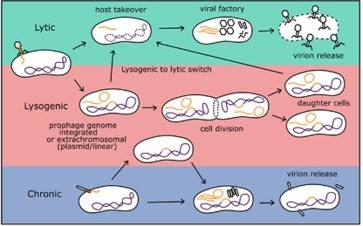
\includegraphics[width=0.4\textwidth]{./figures/fig1-lifecycle.jpg}
\caption{Simple schematic representation of the different phage life cycles. \cite{varona2017}} \label{fig1}
\end{center}
\end{figure}

Given their natural predating relationship with bacteria, phages are increasingly gaining traction as potential therapeutic agents in the combat of antibiotic-resistant bacteria, a pressing global health challenge.\cite{ioannou2023,haq2012,gamachu2022,sulakvelidze2001}
%
%
A result of this growing interest in phages creates a pressing need to develop methods to study phages to facilitate identification and classification. 

\subsection{Phage classification}
With the advancements in genomics and metavirunomics, allowing for a more accurate and comprehensive understanding of phage diversity, phage classification has undergone significant changes in recent years, transitioning from a morphological approach to a genomically coherent taxonomical method. The biggest change in the system was the abolishment of former family of tailed phages, caudovirales (Fig~\ref{fig2} \cite{dion2020}), the most abundant group of phages, which was divided into three subfamilies: (i) podoviridae; (ii) myoviridae; and (iii) siphoviridae. In its stead emerged the new class of caudiviricetes, comprised of 4 new orders and 22 new families. \cite{dion2020,turner2021,turner2023,ackermann2007}   
%
%
\begin{figure}
\begin{center}
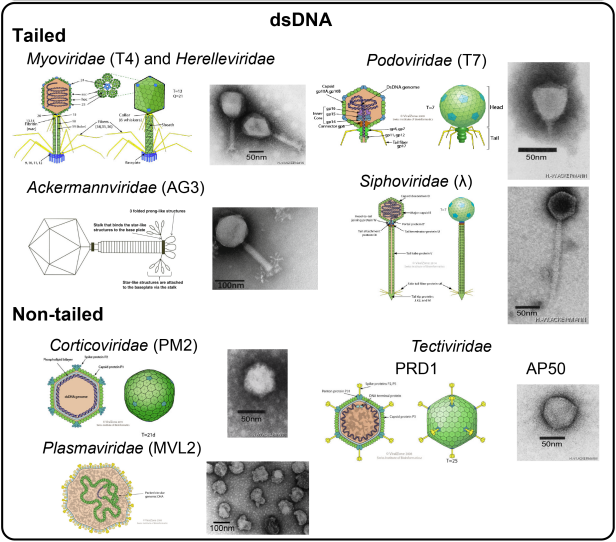
\includegraphics[width=0.4\textwidth]{./figures/fig2-tailed-morpho.png}
\caption{Schematic representation of tailed phages morphology. \cite{dion2020}} \label{fig2}
\end{center}
\end{figure}

%
%
While morphology is no longer used in phage taxonomy, it still retains its importance and impact towards identification and classification and standout as a potential approach for automating tailed phage classification from TEM images. For this work we will use a morphological approach to identify phages based on their morphotype, aiming to identify phage morphotype from TEM images and perform approximate measurements to capsid volume and genome size. There are three distinct tailed phage morphotypes (Fig~\ref{fig3}), based on their respective tailed structures: podoviruses, siphoviruses and myoviruses. \cite{maffei2021} \textbf{Podoviruses} typically display a short non-contractile tail and an icosahedral capsid of about 60 nm in diameter. An example of this virus is \textit{Brucealvirus} CP7R as shown below. \cite{volozhantsev2012} \textbf{Siphoviruses} typically display an icosahedral capsid and a long, flexible but non-contractile tail, spiked at the tip. An example if this morphotype, BlueFeather, can be seen below. \cite{demo2021} \textbf{Myoviruses} display a contractile tail with a base plate and spikes at the tip and an icosahedral capsid. One example of this viruses is \textit{Synechococcus} Phage S-PM2. \cite{mann2005}

\begin{figure}
    
    \begin{subfigure}[b]{0.3\textwidth}
        \begin{center}
        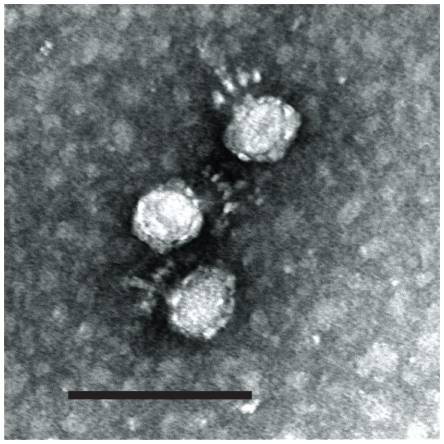
\includegraphics[height = 100px]{./figures/fig-3-1-podovirus.jpg}
        \caption{Podovirus}
        \end{center}
    \end{subfigure}
    \hfill
    \begin{subfigure}[b]{0.3\textwidth}
    \begin{center}
        
    
        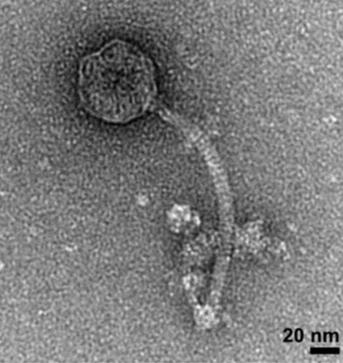
\includegraphics[height = 100px]{./figures/fig-3-2-siphovirus.jpeg}
        \caption{Siphovirus}
        \end{center}
    \end{subfigure}
    \hfill
    \begin{subfigure}[b]{0.3\textwidth}
    \begin{center}
        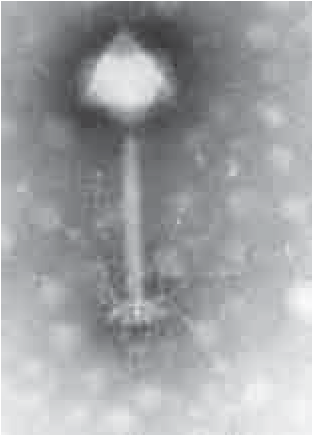
\includegraphics[height = 100px]{./figures/fig-3-3-myovirus.png}
        \caption{Myovirus}
        \end{center}
    \end{subfigure}
    \caption{Morphotypes of phages present in the caudoviricetes class, the most abundant class of phages in the currently existing knowledge. From left to right are shown specimens of podovirus CP7R, a Chlostridium perfringens phage, siphovirus BlueFeather, a Arthrobacter globiformis phage, and myovirus S-PM2, a Synecochus sp. phage. \cite{volozhantsev2012,demo2021,mann2005}}
    \label{fig3}
\end{figure}
As for viral particle size, specifically capsid sizes, these can range from 30 nm to 180nm, enveloping genomes of varying sizes and complexities. \cite{luque2020,lee2022} While there is no clear consensus about the direct correlation between genome and capsid sizes, several authors have been registering a generally accepted allometric relationship between genome length and capsid volume. For the sake of this study we will consider a ratio of 1.52 capsid volume: genome length, being this the adjusted exponent found for dsDNA viruses, specifically tailed phages. \cite{luque2020,lee2022,cui2014,chaudhari2021} 

\subsection{Automated viral particle detection and classification}

Automatic detection and recognition of particles from digital microscopy images is still an active yet unexplored field.
One of the main advantages of developing accurate and efficient methods for automatic detection of viral particles is the automation of the fastidious and labour-intensive work associated with microscope analysis - safeguarding the impact that human factors such as fatigue can have on the analysis (be it counting or identifying particle types).  \cite{glaeser2004}  This is also the case for automatic recognition of viral particles, where qualitative and quantitative measurements involve processing hundreds or thousands of microscopy images to count particles and identify viral morphotypes. \cite{glaeser2004,gelzinis2015}

It is accepted that in order to be regarded as valuable, automatic recognition systems must attain an accuracy greater than 75\% when compared to a human expert. \cite{glaeser2004} There are notable methods in the literature for automatic particle identification using machine learning techniques such as neural networks, Gaussian classifiers, Naive Bayes, and random forests that have achieved this requisite to different degrees. \cite{gelzinis2015,ogura2004,sorzano2009,castanon2007}

Each of these techniques exhibit different advantages and disadvantages considering the scenarios and data at hand, for instance: Gaussian classifiers, operating as statistical models, excel at classifying image features assuming a Gaussian distribution. These classifiers assess the probability of each data point belonging to a specific class based on its features and assign it to the most probable class. They are particularly effective when handling images with features that adhere to a normal distribution and classes that are distinctly separated. \cite{xu2022}

Random forests, on the other hand, are ensemble learning approaches that can be used for classification and regression. Each decision tree in the ensemble is trained on a random subset of the training data and features. During prediction, the forest's trees separately anticipate the class of the incoming data, with the final prediction established by a majority vote or averaging across all trees. Random forests, which are well-known for their resistance to over fitting, are especially useful when dealing with heterogeneous datasets. \cite{caie2021} 

Naive Bayes, despite its simplicity, emerges as a powerful probabilistic classifier. It operates under the assumption of feature independence, calculating class probabilities based on the input image data and selecting the class with the highest probability as the prediction. While straightforward, Naive Bayes demonstrates remarkable proficiency, especially in scenarios involving image classification tasks. \cite{desouza2022} 

Finally, neural networks, specifically convolutional neural networks (CNNs) inspired by the human brain, stand as versatile models for image analysis. Through interconnected layers of nodes, neural networks learn complex patterns and relationships within images by adjusting connection weights during training. Their adaptability and capability to discern intricate patterns have propelled their success across various domains, including image recognition and particle identification. \cite{teuwen2020}

\section{Methods/approach}

This work aims to explore Machine Learning (ML) and Deep Learning (DL) techniques and develop a novel tool - PhageScan - to classify phages, more specifically, we to evaluate the employment of CNNs in automated phage particle recognition given their versatility and high level of discernment for image classification with high accuracy. \cite{ogura2004} More specifically we will explore and evaluate the application of \href{https://docs.ultralytics.com/models/yolov8/}{You Only Look Once (YOLO)} algorithms. YOLO was created as an approach for object detection and has been demonstrating growing accuracy and real-time performance and have already been employed in the field of biological images processing. \cite{li2023,zhu2023,gonzalez2023}

It is important to refer the existence of several challenges for the development of this tool namely: (i) the lack of publicly available data sets of phage TEM micrographs, the existing phage micrographs are sparse and spread throughout data bases and / or closed access publications, thus raising copyright issues; (ii) the quality of available TEM micrographs, which tipically have high levels of noise and require severe processing; (iii) the lack of a good variety of micrographs of phages in their environment, namely multiple phages and hosts on a sample; (iv) podoviruses exhibit small tails that could be confused be hard to detect; (v) myoviruses' tails have a contracted / relaxed state, adding complexity to labelling and classification. On the other hand, siphoviruses, with their relatively consistant capsid shape and long non-contractile tails, are a good starting point, moreover siphoviruses are the most abundant morphotype. 

\subsection{Data gathering, preprocessing and labelling}

\subsubsection{Data gathering}

The success of training an object-detection algorithm such as YOLOv8 lies deeply in the amount and quality of the data set that is presented to the model. As such, it is crucial to have an extensive and diverse range of images that adequately represent the variability and complexity of scenarios in which the tool will be used. 
Specifically, it is fundamental to gather large amounts of TEM micrographs of isolated siphoviruses, siphoviruses and bacteria (infection scenario for example), siphoviruses and other phage types, among other scenarios. Having this diversity and consistency ensures better contextual identification of myoviruses, reduces false positives and ensures better accuracy. This in itself is a challenging undertaking as TEM micrographs with these specific scenarios are relatively scarce. As such, on a first approach we will be sourcing TEM micrographs from curated databases such as \href{https://phagesdb.org/}{PhagesDB} which has a repertoire of 243 phages with TEM images 119 of which belonging to the siphovirus morphotype. Existing literature studying specific myoviruses can also be a source.

\subsection{Preprocessing, augmentation and annotation}
Once the data set creation is achieved, the next step is to preprocess the data, ensuring the consistency and quality of the images contained by the data set through resizing images to a fixed size, ensuring all scales are correctly represented, adjusting image quality (brightness, contrast, noise and artifact removal). The data set will also be augmented through \href{https://blog.roboflow.com/why-and-how-to-implement-random-rotate-data-augmentation/}{random rotations and flips} in order to create scenarios where the target objects of classification and identification can be identified independently from image rotation angle, being this a common data augmentation approach for object detection algorithms. \cite{gonzalez2023} 

Finally, to make the data set presentable to the algorithm, it’s fundamental to annotate the images in order to specify what is what. This process is achieved through specifying object classes and location within the images with bounding boxes. This can be achieved using tools such as using tools such as \href{https://pypi.org/project/labelImg/1.4.0/}{LabelImg} or \href{https://docs.ultralytics.com/integrations/roboflow/}{Roboflow}, being the latter well documented in the context of data set preparation and annotation for YOLO algorithms. The annotation process for phages can follow different approaches: (i) draw a bounding box directly on top of the phage, the simplest approach to classify phages in micrographs where there are other objects present; (ii) separating phages into two sub-classes: head and tail, particularly relevant for images of isolated phages, increasing context in micrographs where could exist other objects with strong contrast resembling the head such as bacteria. Considering we will be dealing with TEM micrographs, cases in which there are images with high amounts of noise and incorrect contrast levels could arise. This would imply considering the application of more complex image processing techniques typically used in computational analysis of microscopy images, such as edge detection/filtering, pixel intensity interpolation. These techniques refine the image in order to make the phage objects (head and tail) more visible. \cite{sorzano2009} It is important to reserve smaller, unannotated subsets of the dataset to serve as validation and testing sets, respectively. This allows for an accurate assessment of the algorithm's effectiveness in training, validation, and generalization to unseen data.

\subsection{Model training}

Two object detection architectures will be tested: YOLOv5 and YOLOv8. The models will then be trained on the generated data set for a varying number of epochs in order to empirically determine the best training settings and compare results for both algorithms in order to find the most efficient for the desired application. For this comparison, we will be evaluating and comparing the models' performance, namely by analysing each model's accuracy, precision, recall, F1-Scores and confusion matrices. Once the classification component of the tool is working with a satisfactory accuracy we will then move on to the implementation of automatic capsid annotation and measurement for genome size estimation. 

\newpage
%
% ---- Bibliography ----
%
% BibTeX users should specify bibliography style 'splncs04'.
% References will then be sorted and formatted in the correct style.
%
%\bibliographystyle{splncs04}
\bibliographystyle{unsrt}
\bibliography{bibliography}
%

\end{document}
